%==============================================================================
%  CMPE 492 — A0 landscape research poster (beamerposter)
%  Synthetic Benchmark Generation & Retriever Fine-Tuning for a RAG Trainer
%  Compile:  latexmk -pdf poster.tex   (auto-runs bibtex for references.bib)
%            or:  pdflatex -> bibtex -> pdflatex -> pdflatex
%  3 columns, no footer, thin header:
%    COL1 = What We Do + Results (peak)   COL2 = Pipeline   COL3 = everything else
%  References block still holds [TODO] placeholders — fill citations later.
%==============================================================================
\documentclass[final]{beamer}

\usepackage[size=a0,orientation=landscape,scale=1.0]{beamerposter}
\usetheme{default}
\usepackage[T1]{fontenc}
\usepackage[utf8]{inputenc}
\usepackage{lmodern}
\usepackage{anyfontsize}
\usepackage{graphicx}
\usepackage{tcolorbox}
\tcbuselibrary{skins}
\usepackage{enumitem}
\usepackage{ragged2e}
\usepackage{multicol}

\graphicspath{{./}}

%--- Boğaziçi colour palette --------------------------------------------------
\definecolor{bounnavy}{HTML}{0B2C66}
\definecolor{bounblue}{HTML}{1B4DA0}
\definecolor{bounsky}{HTML}{6FA8DC}
\definecolor{bounlight}{HTML}{EEF3FB}
\definecolor{accgreen}{HTML}{2E8B57}
\definecolor{accred}{HTML}{C0392B}

\setbeamercolor{background canvas}{bg=white}

% numbered references, no icon, compact — pulled from references.bib via bibtex
\setbeamertemplate{bibliography item}{\insertbiblabel}
\setbeamercolor{bibliography item}{fg=bounnavy}
\setbeamercolor{bibliography entry author}{fg=black}
\setbeamercolor{bibliography entry title}{fg=black}
\setbeamercolor{bibliography entry location}{fg=black}
\setbeamercolor{bibliography entry note}{fg=black}

%--- Font sizes ---------------------------------------------------------------
\newcommand{\TitleFont}{\fontsize{68}{76}\selectfont}
\newcommand{\MetaFont}{\fontsize{29}{36}\selectfont}
\newcommand{\BlockTitleFont}{\bfseries\fontsize{36}{44}\selectfont}
\newcommand{\BodyFont}{\fontsize{25}{32}\selectfont}     % introduction
\newcommand{\MethFont}{\fontsize{23}{29}\selectfont}     % methodology
\newcommand{\ConclFont}{\fontsize{24}{31}\selectfont}    % conclusions / future work
\newcommand{\SetupFont}{\fontsize{22}{27}\selectfont}    % models & setup
\newcommand{\RefFont}{\fontsize{20}{25}\selectfont}
\newcommand{\CaptFont}{\itshape\fontsize{19}{24}\selectfont}

%--- Block style --------------------------------------------------------------
\tcbset{
  posterblock/.style={
    enhanced,
    colback=white,
    colframe=bounnavy,
    coltitle=white,
    colbacktitle=bounnavy,
    fonttitle=\BlockTitleFont,
    fontupper=\BodyFont,
    boxrule=2pt,
    arc=7mm,
    left=10mm,right=10mm,top=5mm,bottom=5mm,
    toptitle=3mm,bottomtitle=3mm,
    boxsep=1mm,
    titlerule=0mm,
    halign title=left,
    width=\linewidth,
  }
}
\newtcolorbox{pblock}[1]{posterblock,title={#1}}
% accent blocks now use the same navy as the header (was bounblue)
\newtcolorbox{pblockaccent}[1]{posterblock,title={#1}}

\setlist[itemize]{leftmargin=9mm,itemsep=2.4mm,topsep=1.5mm,parsep=0mm,
  label=\textcolor{bounblue}{\textbf{\textbullet}}}
\setlist[enumerate]{leftmargin=12mm,itemsep=2.4mm,topsep=1.5mm,parsep=0mm,
  label=\protect\colorbox{bounblue}{\makebox[7mm][c]{\color{white}\bfseries\arabic*}}}
\newcommand{\subhd}[1]{\smallskip\textbf{\color{bounblue}#1}\par\nopagebreak}
\newcommand{\lbl}[1]{\textbf{\color{bounblue}#1}}

\newcommand{\todo}[1]{{\color{accred}\textbf{[#1]}}}

% identical header logo (white rounded box, centred) — used in BOTH top corners
\newcommand{\logobox}{%
  \begin{tcolorbox}[colback=white,colframe=white,arc=6mm,boxrule=0pt,
      left=5mm,right=5mm,top=5mm,bottom=5mm,width=\linewidth,
      halign=center,valign=center]
    
\includegraphics[width=0.92\linewidth]{boun-logo-clean.png}
  \end{tcolorbox}}

\begin{document}
\begin{frame}[t]
%==============================================================================
%  THIN HEADER BAND — logos both corners, meta on one line
%==============================================================================
\begin{tcolorbox}[enhanced,colback=bounnavy,colframe=bounnavy,boxrule=0pt,
    arc=8mm,left=16mm,right=16mm,top=7mm,bottom=7mm,width=\linewidth]
\begin{columns}[c]
  \begin{column}{0.12\linewidth}\centering\logobox\end{column}
  \begin{column}{0.74\linewidth}
    \centering\color{white}
    {\TitleFont\bfseries Making RAG Systems Domain-Specific by Fine-Tuning\\[3mm]
     Embedders on Synthetic Queries\par}
    \vspace{6mm}
    {\MetaFont CMPE 492 \;\textbullet\; Hikmet Can Köseoğlu
     \;\textbullet\; Advisor: Bahri Atay Özgövde \;\textbullet\;
     Dept.\ of Computer Engineering, Boğaziçi University\par}
  \end{column}
  \begin{column}{0.12\linewidth}\centering\logobox\end{column}
\end{columns}
\end{tcolorbox}

\vspace{3mm}

%==============================================================================
%  THREE-COLUMN BODY
%  COL1 : What We Do + Results (peak bars)
%  COL2 : Pipeline Overview (pipeline.jpg)
%  COL3 : everything else — Intro, Methodology, Models, Conclusions, Future, Refs
%==============================================================================
\begin{columns}[t,onlytextwidth]
%---------------------------- COL 1 : INTRO + METHOD + WHAT WE DO + PEAK ------
\begin{column}{0.30\linewidth}
  \begin{pblock}{Introduction}
    \BodyFont\justifying
    \lbl{PROBLEM:} The quality of any RAG system is bounded by its retriever. If the
    passage that contains the answer is not retrieved into the top-$k$, no amount of
    generation skill can recover the correct response -- retrieval failure is an upper
    bound on end-to-end accuracy.

    \smallskip
    \lbl{AIM:} We generate a synthetic, in-domain training set from fitness literature,
    then fine-tune embedding retrievers of different sizes on it and measure the
    improvement over their off-the-shelf baselines.
  \end{pblock}

  \vspace{4mm}

  \begin{pblock}{Methodology}
    \MethFont\justifying
    \subhd{A) Benchmark Creation}
    \begin{enumerate}
      \item Parse each document into self-contained statements (propositions).
      \item Group consecutive statements into semantically coherent, variable-length
            chunks.
      \item Generate two queries per chunk (formal + informal); a judge verifies each and
            regenerates failures with feedback.
      \item Hybrid search (dense + keyword/BM25) retrieves candidate chunks for each query.
      \item A judge labels each candidate \textbf{positive}, \textbf{hard-negative}, or
            \textbf{irrelevant}.
    \end{enumerate}
    \subhd{B) Fine-Tuning}
    \begin{enumerate}[start=6]
      \item Train the embedder on \textbf{(query, positive, hard-negative)} triplets --
            positives pull closer, hard-negatives push away. Split by query to prevent
            leakage.
    \end{enumerate}
  \end{pblock}

  \vspace{4mm}

  \begin{pblockaccent}{What We Do}
    \centering
    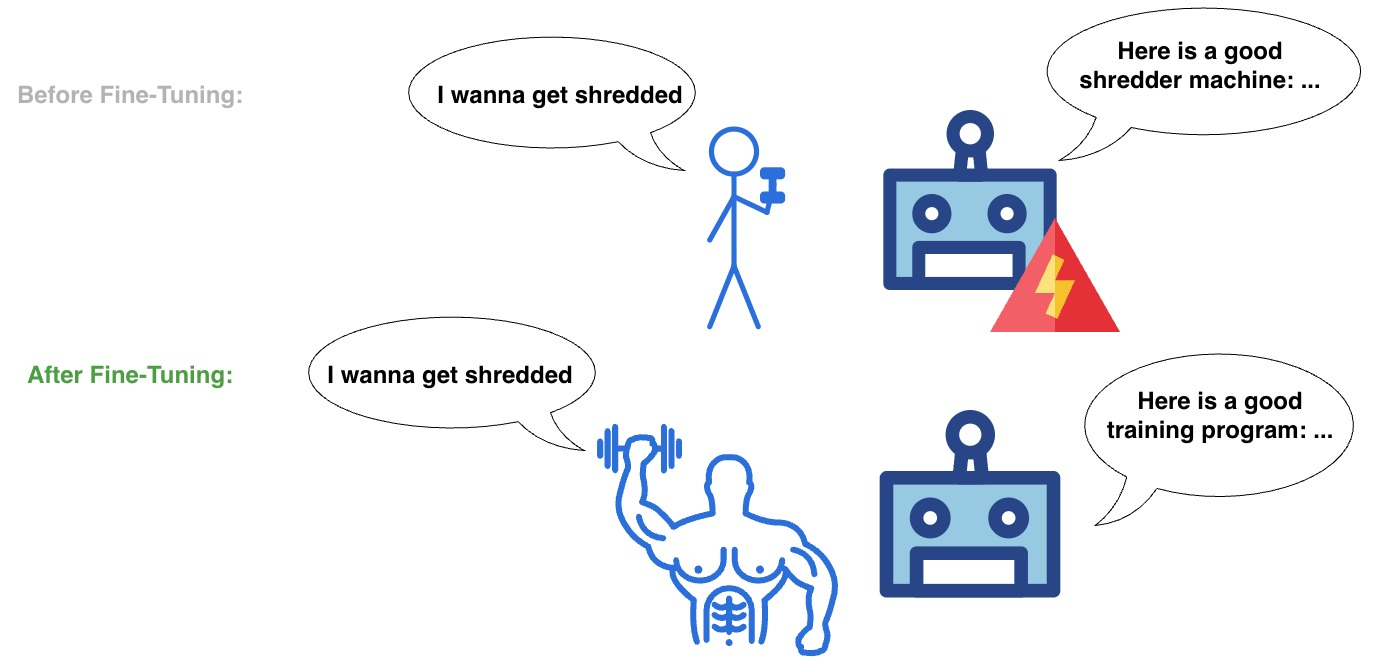
\includegraphics[width=0.92\linewidth]{what_we_do.jpg}
  \end{pblockaccent}

  \vspace{4mm}

  \begin{pblockaccent}{Results}
    \centering
    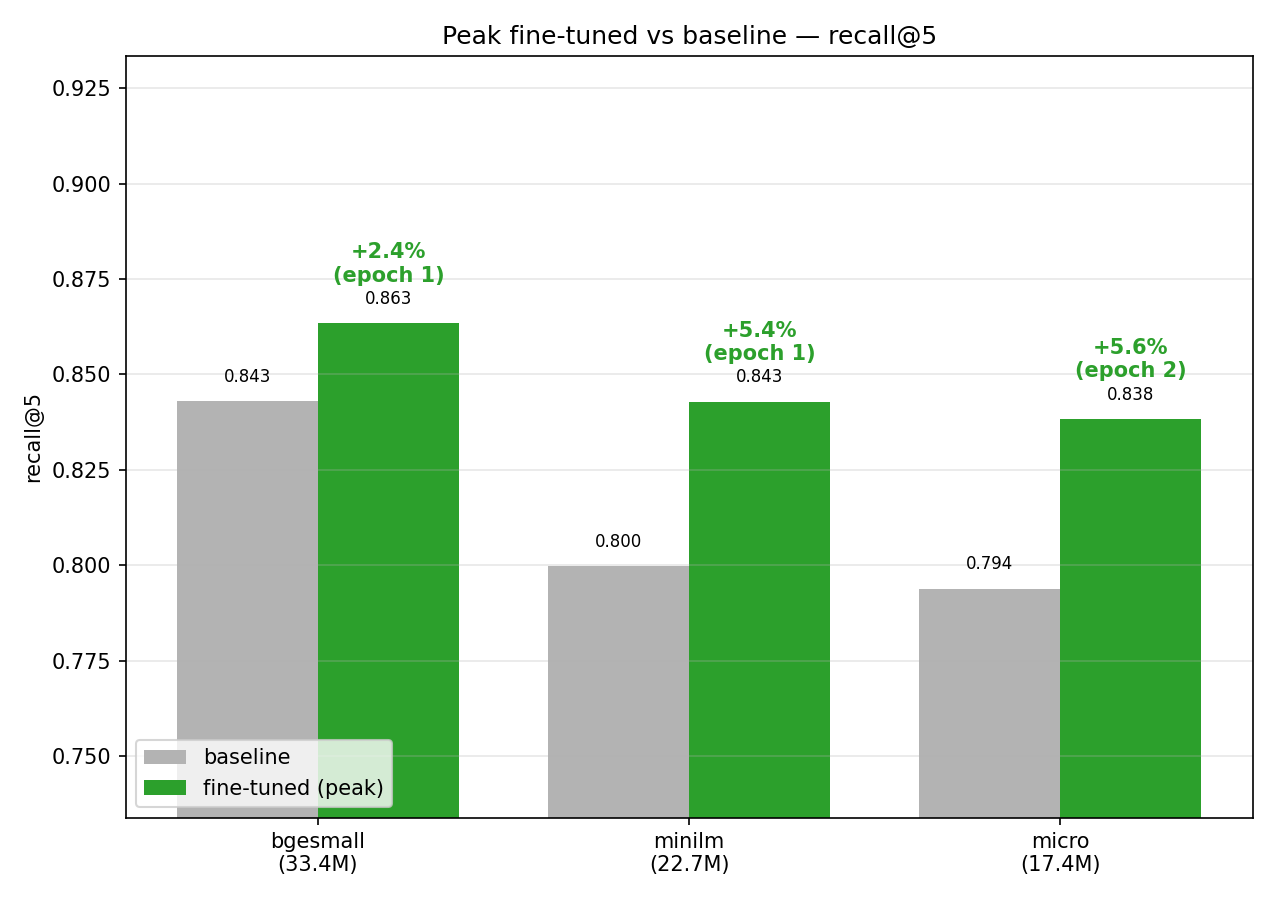
\includegraphics[width=0.53\linewidth]{peak_vs_baseline_recall5.png}\\[1mm]
    {\CaptFont Peak fine-tuned vs.\ baseline (Recall@5): every model improves.}
  \end{pblockaccent}
\end{column}
%---------------------------- COL 2 : PIPELINE (bigger) ----------------------
\begin{column}{0.34\linewidth}
  \begin{pblockaccent}{Pipeline Overview}
    \centering
    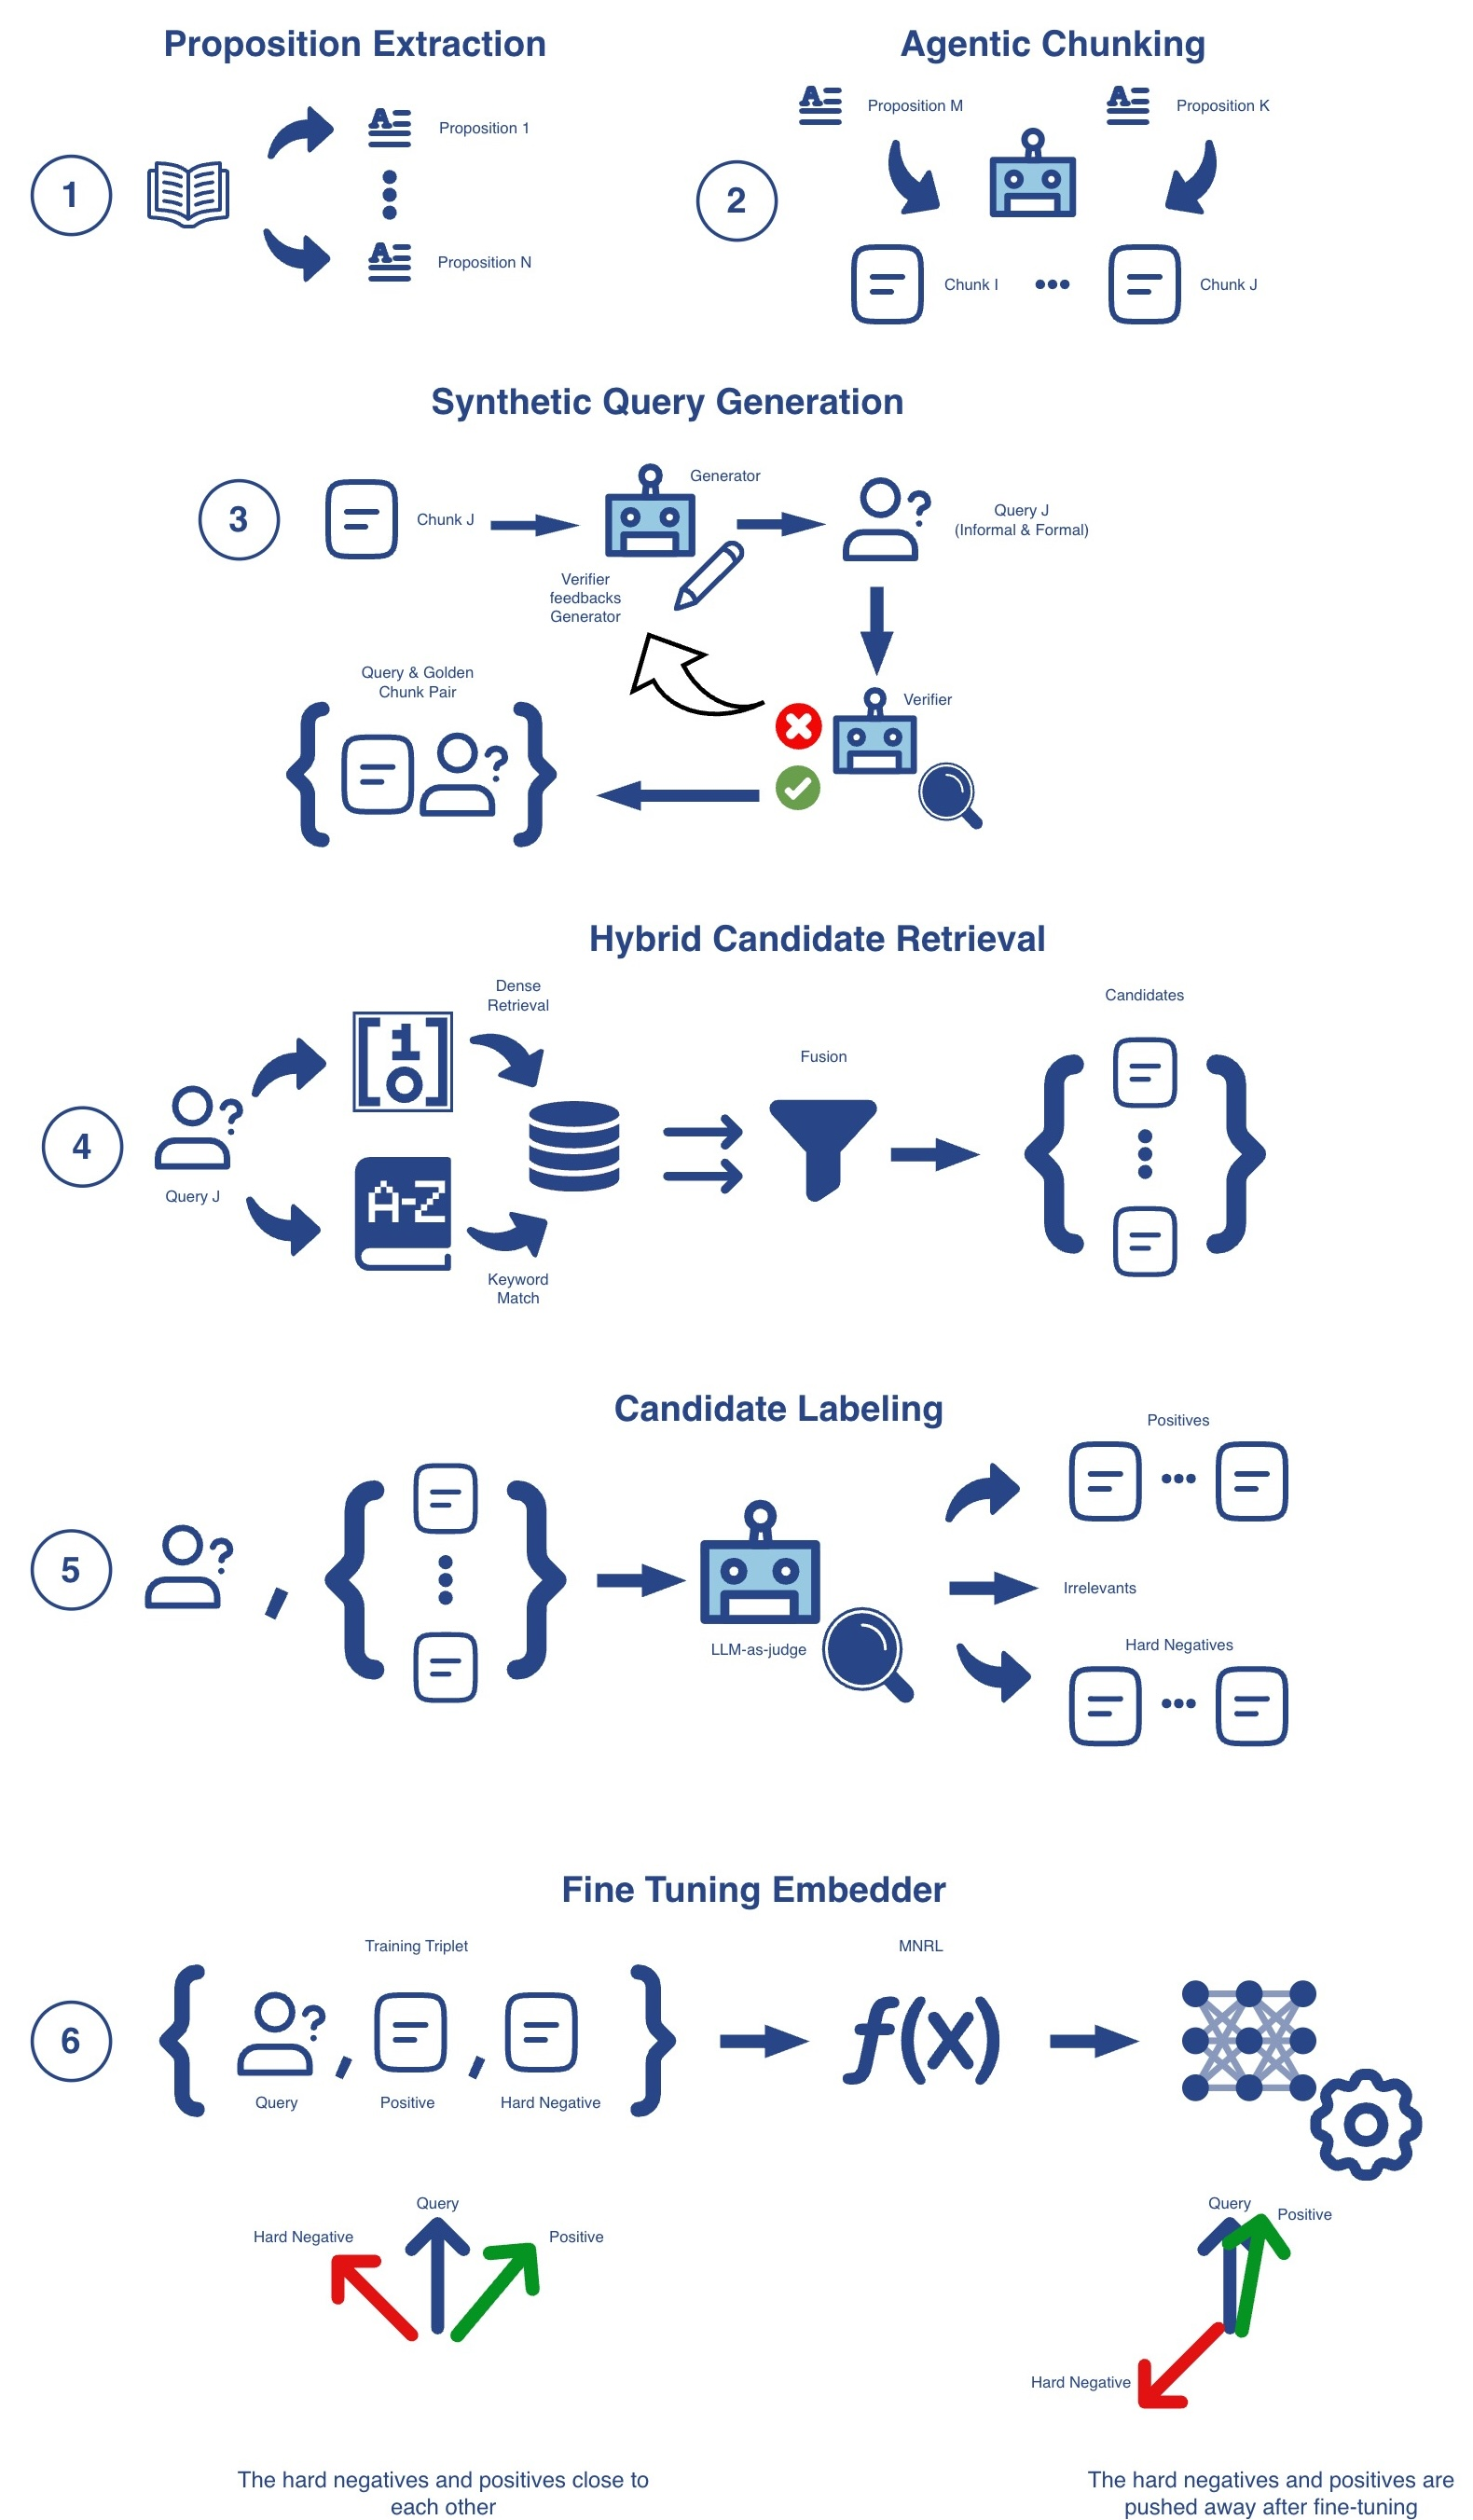
\includegraphics[width=0.95\linewidth]{pipeline.jpg}
  \end{pblockaccent}
\end{column}
%---------------------------- COL 3 : EVERYTHING ELSE ------------------------
\begin{column}{0.36\linewidth}
  \begin{pblock}{Models \& Setup}
    \SetupFont
    \lbl{Hardware.} Data generation on \textbf{NVIDIA L4 (24\,GB, GCP)} via vLLM;
    fine-tuning on a local \textbf{Apple M1 (16\,GB)}.\par\smallskip
    \lbl{Pipeline.} Generator \textbf{Gemma 2 9B Instruct} (4-bit); judge
    \textbf{DeepSeek-R1-0528-Qwen3-8B} for reasoning-based hard-negative validation.\par\smallskip
    \lbl{Retrievers.} bge-small (33.4M), all-MiniLM-L6-v2 (22.7M), bge-micro (17.4M).\par\smallskip
    \lbl{Training \& eval.} MNRL loss, batch 16, lr 2e-5, 1--3 epochs; Recall@1/5/10 and
    NDCG@10 with 95\% CIs.
  \end{pblock}

  \vspace{4mm}

  \begin{pblockaccent}{Results (cont.)}
    \centering
    \begin{columns}[t,onlytextwidth]
      \begin{column}{0.49\linewidth}\centering
        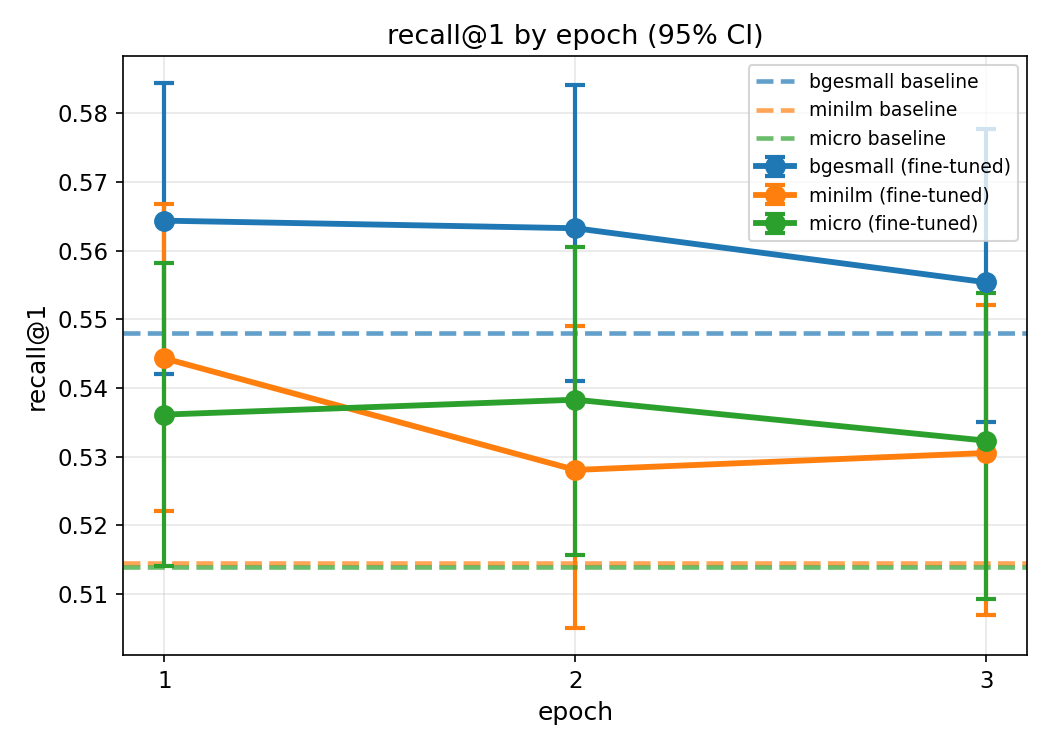
\includegraphics[width=0.82\linewidth]{overall_recall1.png}\\[2mm]
        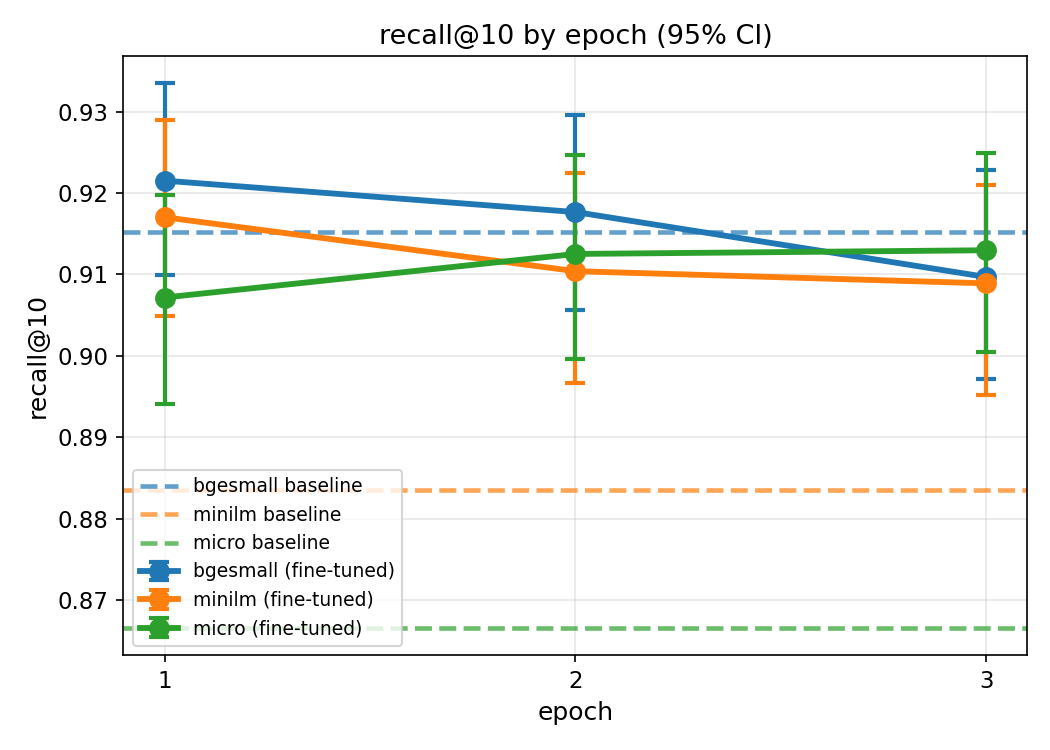
\includegraphics[width=0.82\linewidth]{overall_recall10.png}
      \end{column}
      \begin{column}{0.49\linewidth}\centering
        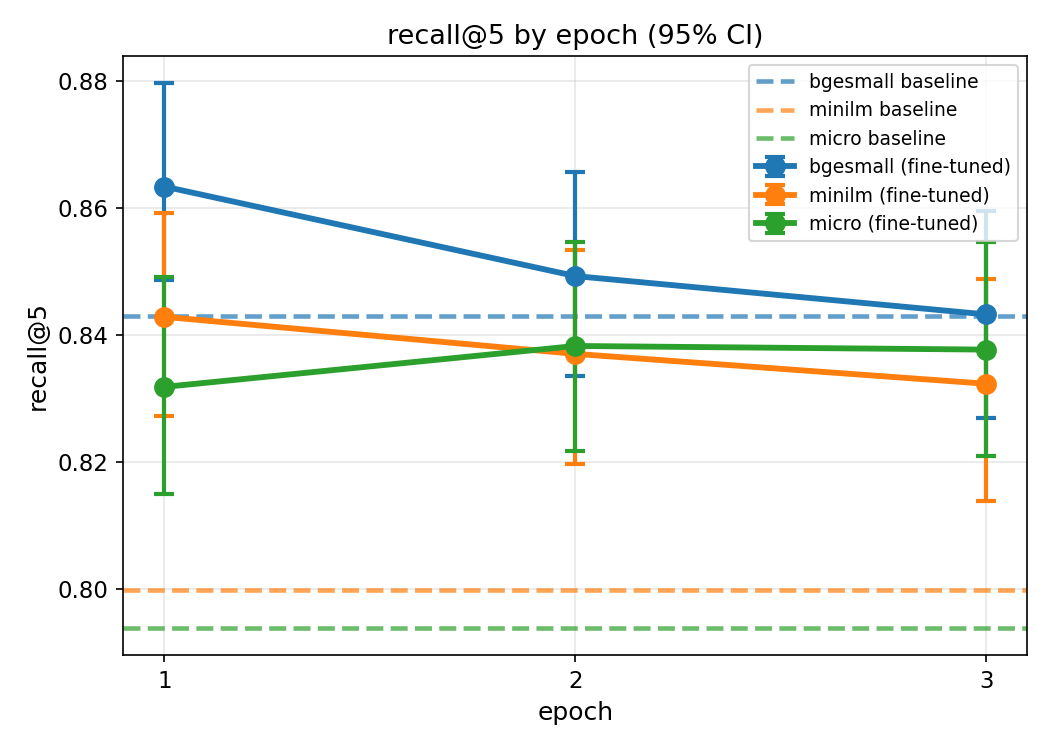
\includegraphics[width=0.82\linewidth]{overall_recall5.png}\\[2mm]
        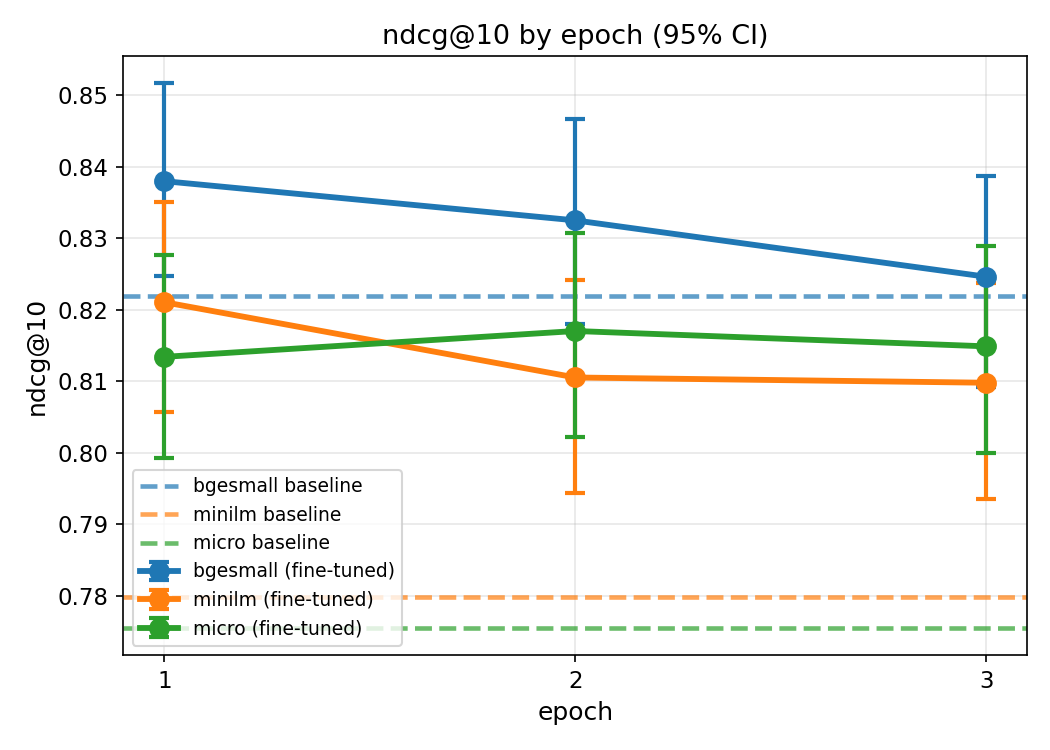
\includegraphics[width=0.82\linewidth]{overall_ndcg10.png}
      \end{column}
    \end{columns}
  \end{pblockaccent}

  \vspace{4mm}

  \begin{pblock}{Conclusions}
    \ConclFont
    \begin{itemize}
      \item Fine-tuning on synthetic in-domain triplets \textbf{beats the off-the-shelf
            baseline for every retriever}.
      \item Smaller, weaker bases gain the most (more headroom): bge-micro cuts top-5
            retrieval misses $\sim$21\% and top-10 misses $\sim$35\%.
      \item Optimal training is short: bge-small and all-MiniLM peak at epoch 1, bge-micro at
            epoch 2; beyond the peak they overfit.
    \end{itemize}
  \end{pblock}

  \vspace{4mm}

  \begin{pblock}{Future Work}
    \ConclFont
    \begin{itemize}
      \item \textbf{Standardized benchmark:} evaluate on a public suite (e.g.\ BEIR) to
            measure out-of-domain forgetting.
      \item \textbf{Multi-hop questions:} extend the data and metrics to queries that need
            several passages.
      \item \textbf{Early stopping \& regularization:} train longer without overfitting past
            the peak epoch.
    \end{itemize}
  \end{pblock}

  \vspace{4mm}

  \begin{pblock}{References}
    {\fontsize{14}{17}\selectfont
     \bibliographystyle{ieeetr}\nocite{*}
     \setlength{\columnsep}{7mm}
     \begin{multicols}{2}\raggedright
       \bibliography{references}
     \end{multicols}}
  \end{pblock}
\end{column}
\end{columns}

\end{frame}
\end{document}
